\documentclass[journal,12pt,twocolumn]{IEEEtran}
%
\usepackage{setspace}
\usepackage{gensymb}
\usepackage{xcolor}
\usepackage{caption}
%\usepackage{subcaption}
%\doublespacing
\singlespacing

%\usepackage{graphicx}
%\usepackage{amssymb}
%\usepackage{relsize}
\usepackage[cmex10]{amsmath}
\usepackage{mathtools}
%\usepackage{amsthm}
%\interdisplaylinepenalty=2500
%\savesymbol{iint}
%\usepackage{txfonts}
%\restoresymbol{TXF}{iint}
%\usepackage{wasysym}
\usepackage{amsthm}
\usepackage{mathrsfs}
\usepackage{txfonts}
\usepackage{stfloats}
\usepackage{cite}
\usepackage{cases}
\usepackage{subfig}
%\usepackage{xtab}
\usepackage{longtable}
\usepackage{multirow}
%\usepackage{algorithm}
%\usepackage{algpseudocode}
\usepackage{enumitem}
\usepackage{mathtools}
\usepackage{eenrc}
%\usepackage[framemethod=tikz]{mdframed}
\usepackage{hyperref}
\usepackage{listings}
    \usepackage[latin1]{inputenc}                                 %%
    \usepackage{color}                                            %%
    \usepackage{array}                                            %%
    \usepackage{longtable}                                        %%
    \usepackage{calc}                                             %%
    \usepackage{multirow}                                         %%
    \usepackage{hhline}                                           %%
    \usepackage{ifthen}                                           %%
  %optionally (for landscape tables embedded in another document): %%
    \usepackage{lscape}     
\usepackage{tikz}
\usepackage{circuitikz}
\usepackage{karnaugh-map}
\usepackage{pgf}

\usepackage{url}
\def\UrlBreaks{\do\/\do-}



%\usepackage{stmaryrd}


%\usepackage{wasysym}
%\newcounter{MYtempeqncnt}
\DeclareMathOperator*{\Res}{Res}
%\renewcommand{\baselinestretch}{2}
\renewcommand\thesection{\arabic{section}}
\renewcommand\thesubsection{\thesection.\arabic{subsection}}
\renewcommand\thesubsubsection{\thesubsection.\arabic{subsubsection}}

\renewcommand\thesectiondis{\arabic{section}}
\renewcommand\thesubsectiondis{\thesectiondis.\arabic{subsection}}
\renewcommand\thesubsubsectiondis{\thesubsectiondis.\arabic{subsubsection}}

% correct bad hyphenation here
\hyphenation{op-tical net-works semi-conduc-tor}

%\lstset{
%language=C,
%frame=single, 
%breaklines=true
%}

%\lstset{
	%%basicstyle=\small\ttfamily\bfseries,
	%%numberstyle=\small\ttfamily,
	%language=Octave,
	%backgroundcolor=\color{white},
	%%frame=single,
	%%keywordstyle=\bfseries,
	%%breaklines=true,
	%%showstringspaces=false,
	%%xleftmargin=-10mm,
	%%aboveskip=-1mm,
	%%belowskip=0mm
%}

%\surroundwithmdframed[width=\columnwidth]{lstlisting}
\def\inputGnumericTable{}                                 %%
\lstset{
%language=C,
frame=single, 
breaklines=true,
columns=fullflexible
}
 

\begin{document}
%

\theoremstyle{definition}
\newtheorem{theorem}{Theorem}[section]
\newtheorem{problem}{Problem}
\newtheorem{proposition}{Proposition}[section]
\newtheorem{lemma}{Lemma}[section]
\newtheorem{corollary}[theorem]{Corollary}
\newtheorem{example}{Example}[section]
\newtheorem{definition}{Definition}[section]
%\newtheorem{algorithm}{Algorithm}[section]
%\newtheorem{cor}{Corollary}
\newcommand{\BEQA}{\begin{eqnarray}}
\newcommand{\EEQA}{\end{eqnarray}}
\newcommand{\define}{\stackrel{\triangle}{=}}

\bibliographystyle{IEEEtran}
%\bibliographystyle{ieeetr}

\providecommand{\nCr}[2]{\,^{#1}C_{#2}} % nCr
\providecommand{\nPr}[2]{\,^{#1}P_{#2}} % nPr
\providecommand{\mbf}{\mathbf}
\providecommand{\pr}[1]{\ensuremath{\Pr\left(#1\right)}}
\providecommand{\qfunc}[1]{\ensuremath{Q\left(#1\right)}}
\providecommand{\sbrak}[1]{\ensuremath{{}\left[#1\right]}}
\providecommand{\lsbrak}[1]{\ensuremath{{}\left[#1\right.}}
\providecommand{\rsbrak}[1]{\ensuremath{{}\left.#1\right]}}
\providecommand{\brak}[1]{\ensuremath{\left(#1\right)}}
\providecommand{\lbrak}[1]{\ensuremath{\left(#1\right.}}
\providecommand{\rbrak}[1]{\ensuremath{\left.#1\right)}}
\providecommand{\cbrak}[1]{\ensuremath{\left\{#1\right\}}}
\providecommand{\lcbrak}[1]{\ensuremath{\left\{#1\right.}}
\providecommand{\rcbrak}[1]{\ensuremath{\left.#1\right\}}}
\providecommand{\ceil}[1]{\left \lceil #1 \right \rceil }
\theoremstyle{remark}
\newtheorem{rem}{Remark}
\newcommand{\sgn}{\mathop{\mathrm{sgn}}}
\providecommand{\abs}[1]{\left\vert#1\right\vert}
\providecommand{\res}[1]{\Res\displaylimits_{#1}} 
\providecommand{\norm}[1]{\lVert#1\rVert}
\providecommand{\mtx}[1]{\mathbf{#1}}
\providecommand{\mean}[1]{E\left[ #1 \right]}
\providecommand{\fourier}{\overset{\mathcal{F}}{ \rightleftharpoons}}
%\providecommand{\hilbert}{\overset{\mathcal{H}}{ \rightleftharpoons}}
\providecommand{\system}{\overset{\mathcal{H}}{ \longleftrightarrow}}
	%\newcommand{\solution}[2]{\textbf{Solution:}{#1}}
\newcommand{\solution}{\noindent \textbf{Solution: }}
\providecommand{\dec}[2]{\ensuremath{\overset{#1}{\underset{#2}{\gtrless}}}}


%\numberwithin{equation}{subsection}
\numberwithin{equation}{problem}
%\numberwithin{problem}{subsection}
%\numberwithin{definition}{subsection}
\makeatletter
\@addtoreset{figure}{problem}
\makeatother

\let\StandardTheFigure\thefigure
%\renewcommand{\thefigure}{\theproblem.\arabic{figure}}
\renewcommand{\thefigure}{\theproblem}


%\numberwithin{figure}{subsection}

%\numberwithin{equation}{subsection}
%\numberwithin{equation}{section}
%%\numberwithin{equation}{problem}
%%\numberwithin{problem}{subsection}
\numberwithin{problem}{section}
%%\numberwithin{definition}{subsection}
%\makeatletter
%\@addtoreset{figure}{problem}
%\makeatother
\makeatletter
\@addtoreset{table}{problem}
\makeatother

\let\StandardTheFigure\thefigure
\let\StandardTheTable\thetable
%%\renewcommand{\thefigure}{\theproblem.\arabic{figure}}
%\renewcommand{\thefigure}{\theproblem}
\renewcommand{\thetable}{\theproblem}
%%\numberwithin{figure}{section}

%%\numberwithin{figure}{subsection}



\def\putbox#1#2#3{\makebox[0in][l]{\makebox[#1][l]{}\raisebox{\baselineskip}[0in][0in]{\raisebox{#2}[0in][0in]{#3}}}}
     \def\rightbox#1{\makebox[0in][r]{#1}}
     \def\centbox#1{\makebox[0in]{#1}}
     \def\topbox#1{\raisebox{-\baselineskip}[0in][0in]{#1}}
     \def\midbox#1{\raisebox{-0.5\baselineskip}[0in][0in]{#1}}

\vspace{3cm}

\title{ 
	\logo{
	Decade Counter through 7474
	}
}



% paper title
% can use linebreaks \\ within to get better formatting as desired
%\title{Matrix Analysis through Octave}
%
%
% author names and IEEE memberships
% note positions of commas and nonbreaking spaces ( ~ ) LaTeX will not break
% a structure at a ~ so this keeps an author's name from being broken across
% two lines.
% use \thanks{} to gain access to the first footnote area
% a separate \thanks must be used for each paragraph as LaTeX2e's \thanks
% was not built to handle multiple paragraphs
%

\author{G V V Sharma$^{*}$% <-this % stops a space
\thanks{*The author is with the Department
of Electrical Engineering, Indian Institute of Technology, Hyderabad
502285 India e-mail:  gadepall@iith.ac.in. All content in this manual is released under GNU GPL.  Free and open source.}% <-this % stops a space
%\thanks{J. Doe and J. Doe are with Anonymous University.}% <-this % stops a space
%\thanks{Manuscript received April 19, 2005; revised January 11, 2007.}}
}
% note the % following the last \IEEEmembership and also \thanks - 
% these prevent an unwanted space from occurring between the last author name
% and the end of the author line. i.e., if you had this:
% 
% \author{....lastname \thanks{...} \thanks{...} }
%                     ^------------^------------^----Do not want these spaces!
%
% a space would be appended to the last name and could cause every name on that
% line to be shifted left slightly. This is one of those "LaTeX things". For
% instance, "\textbf{A} \textbf{B}" will typeset as "A B" not "AB". To get
% "AB" then you have to do: "\textbf{A}\textbf{B}"
% \thanks is no different in this regard, so shield the last } of each \thanks
% that ends a line with a % and do not let a space in before the next \thanks.
% Spaces after \IEEEmembership other than the last one are OK (and needed) as
% you are supposed to have spaces between the names. For what it is worth,
% this is a minor point as most people would not even notice if the said evil
% space somehow managed to creep in.



% The paper headers
%\markboth{Journal of \LaTeX\ Class Files,~Vol.~6, No.~1, January~2007}%
%{Shell \MakeLowercase{\textit{et al.}}: Bare Demo of IEEEtran.cls for Journals}
% The only time the second header will appear is for the odd numbered pages
% after the title page when using the twoside option.
% 
% *** Note that you probably will NOT want to include the author's ***
% *** name in the headers of peer review papers.                   ***
% You can use \ifCLASSOPTIONpeerreview for conditional compilation here if
% you desire.




% If you want to put a publisher's ID mark on the page you can do it like
% this:
%\IEEEpubid{0000--0000/00\$00.00~\copyright~2007 IEEE}
% Remember, if you use this you must call \IEEEpubidadjcol in the second
% column for its text to clear the IEEEpubid mark.



% make the title area
\maketitle

\tableofcontents

\bigskip

\begin{abstract}
This manual shows how to use the 7474 D-Flip Flop ICs in
a sequential circuit to realize a decade counter.
\end{abstract}
%\newpage
\section{Components}
%\begin{table}[!h]
%\centering
%%%%%%%%%%%%%%%%%%%%%%%%%%%%%%%%%%%%%%%%%%%%%%%%%%%%%%%%%%%%%%%%%%%%%%
%%                                                                  %%
%%  This is the header of a LaTeX2e file exported from Gnumeric.    %%
%%                                                                  %%
%%  This file can be compiled as it stands or included in another   %%
%%  LaTeX document. The table is based on the longtable package so  %%
%%  the longtable options (headers, footers...) can be set in the   %%
%%  preamble section below (see PRAMBLE).                           %%
%%                                                                  %%
%%  To include the file in another, the following two lines must be %%
%%  in the including file:                                          %%
%%        \def\inputGnumericTable{}                                 %%
%%  at the beginning of the file and:                               %%
%%        \input{name-of-this-file.tex}                             %%
%%  where the table is to be placed. Note also that the including   %%
%%  file must use the following packages for the table to be        %%
%%  rendered correctly:                                             %%
%%    \usepackage[latin1]{inputenc}                                 %%
%%    \usepackage{color}                                            %%
%%    \usepackage{array}                                            %%
%%    \usepackage{longtable}                                        %%
%%    \usepackage{calc}                                             %%
%%    \usepackage{multirow}                                         %%
%%    \usepackage{hhline}                                           %%
%%    \usepackage{ifthen}                                           %%
%%  optionally (for landscape tables embedded in another document): %%
%%    \usepackage{lscape}                                           %%
%%                                                                  %%
%%%%%%%%%%%%%%%%%%%%%%%%%%%%%%%%%%%%%%%%%%%%%%%%%%%%%%%%%%%%%%%%%%%%%%



%%  This section checks if we are begin input into another file or  %%
%%  the file will be compiled alone. First use a macro taken from   %%
%%  the TeXbook ex 7.7 (suggestion of Han-Wen Nienhuys).            %%
\def\ifundefined#1{\expandafter\ifx\csname#1\endcsname\relax}


%%  Check for the \def token for inputed files. If it is not        %%
%%  defined, the file will be processed as a standalone and the     %%
%%  preamble will be used.                                          %%
\ifundefined{inputGnumericTable}

%%  We must be able to close or not the document at the end.        %%
	\def\gnumericTableEnd{\end{document}}


%%%%%%%%%%%%%%%%%%%%%%%%%%%%%%%%%%%%%%%%%%%%%%%%%%%%%%%%%%%%%%%%%%%%%%
%%                                                                  %%
%%  This is the PREAMBLE. Change these values to get the right      %%
%%  paper size and other niceties.                                  %%
%%                                                                  %%
%%%%%%%%%%%%%%%%%%%%%%%%%%%%%%%%%%%%%%%%%%%%%%%%%%%%%%%%%%%%%%%%%%%%%%

	\documentclass[12pt%
			  %,landscape%
                    ]{report}
       \usepackage[latin1]{inputenc}
       \usepackage{fullpage}
       \usepackage{color}
       \usepackage{array}
       \usepackage{longtable}
       \usepackage{calc}
       \usepackage{multirow}
       \usepackage{hhline}
       \usepackage{ifthen}

	\begin{document}


%%  End of the preamble for the standalone. The next section is for %%
%%  documents which are included into other LaTeX2e files.          %%
\else

%%  We are not a stand alone document. For a regular table, we will %%
%%  have no preamble and only define the closing to mean nothing.   %%
    \def\gnumericTableEnd{}

%%  If we want landscape mode in an embedded document, comment out  %%
%%  the line above and uncomment the two below. The table will      %%
%%  begin on a new page and run in landscape mode.                  %%
%       \def\gnumericTableEnd{\end{landscape}}
%       \begin{landscape}


%%  End of the else clause for this file being \input.              %%
\fi

%%%%%%%%%%%%%%%%%%%%%%%%%%%%%%%%%%%%%%%%%%%%%%%%%%%%%%%%%%%%%%%%%%%%%%
%%                                                                  %%
%%  The rest is the gnumeric table, except for the closing          %%
%%  statement. Changes below will alter the table's appearance.     %%
%%                                                                  %%
%%%%%%%%%%%%%%%%%%%%%%%%%%%%%%%%%%%%%%%%%%%%%%%%%%%%%%%%%%%%%%%%%%%%%%

\providecommand{\gnumericmathit}[1]{#1} 
%%  Uncomment the next line if you would like your numbers to be in %%
%%  italics if they are italizised in the gnumeric table.           %%
%\renewcommand{\gnumericmathit}[1]{\mathit{#1}}
\providecommand{\gnumericPB}[1]%
{\let\gnumericTemp=\\#1\let\\=\gnumericTemp\hspace{0pt}}
 \ifundefined{gnumericTableWidthDefined}
        \newlength{\gnumericTableWidth}
        \newlength{\gnumericTableWidthComplete}
        \newlength{\gnumericMultiRowLength}
        \global\def\gnumericTableWidthDefined{}
 \fi
%% The following setting protects this code from babel shorthands.  %%
 \ifthenelse{\isundefined{\languageshorthands}}{}{\languageshorthands{english}}
%%  The default table format retains the relative column widths of  %%
%%  gnumeric. They can easily be changed to c, r or l. In that case %%
%%  you may want to comment out the next line and uncomment the one %%
%%  thereafter                                                      %%
\providecommand\gnumbox{\makebox[0pt]}
%%\providecommand\gnumbox[1][]{\makebox}

%% to adjust positions in multirow situations                       %%
\setlength{\bigstrutjot}{\jot}
\setlength{\extrarowheight}{\doublerulesep}

%%  The \setlongtables command keeps column widths the same across  %%
%%  pages. Simply comment out next line for varying column widths.  %%
\setlongtables

\setlength\gnumericTableWidth{%
	133pt+%
	53pt+%
	57pt+%
0pt}
\def\gumericNumCols{3}
\setlength\gnumericTableWidthComplete{\gnumericTableWidth+%
         \tabcolsep*\gumericNumCols*2+\arrayrulewidth*\gumericNumCols}
\ifthenelse{\lengthtest{\gnumericTableWidthComplete > \linewidth}}%
         {\def\gnumericScale{\ratio{\linewidth-%
                        \tabcolsep*\gumericNumCols*2-%
                        \arrayrulewidth*\gumericNumCols}%
{\gnumericTableWidth}}}%
{\def\gnumericScale{1}}

%%%%%%%%%%%%%%%%%%%%%%%%%%%%%%%%%%%%%%%%%%%%%%%%%%%%%%%%%%%%%%%%%%%%%%
%%                                                                  %%
%% The following are the widths of the various columns. We are      %%
%% defining them here because then they are easier to change.       %%
%% Depending on the cell formats we may use them more than once.    %%
%%                                                                  %%
%%%%%%%%%%%%%%%%%%%%%%%%%%%%%%%%%%%%%%%%%%%%%%%%%%%%%%%%%%%%%%%%%%%%%%

\ifthenelse{\isundefined{\gnumericColA}}{\newlength{\gnumericColA}}{}\settowidth{\gnumericColA}{\begin{tabular}{@{}p{133pt*\gnumericScale}@{}}x\end{tabular}}
\ifthenelse{\isundefined{\gnumericColB}}{\newlength{\gnumericColB}}{}\settowidth{\gnumericColB}{\begin{tabular}{@{}p{53pt*\gnumericScale}@{}}x\end{tabular}}
\ifthenelse{\isundefined{\gnumericColC}}{\newlength{\gnumericColC}}{}\settowidth{\gnumericColC}{\begin{tabular}{@{}p{57pt*\gnumericScale}@{}}x\end{tabular}}

\begin{table}[!h]
\begin{tabular}[c]{%
	b{\gnumericColA}%
	b{\gnumericColB}%
	b{\gnumericColC}%
	}

%%%%%%%%%%%%%%%%%%%%%%%%%%%%%%%%%%%%%%%%%%%%%%%%%%%%%%%%%%%%%%%%%%%%%%
%%  The longtable options. (Caption, headers... see Goosens, p.124) %%
%	\caption{The Table Caption.}             \\	%
% \hline	% Across the top of the table.
%%  The rest of these options are table rows which are placed on    %%
%%  the first, last or every page. Use \multicolumn if you want.    %%

%%  Header for the first page.                                      %%
%	\multicolumn{3}{c}{The First Header} \\ \hline 
%	\multicolumn{1}{c}{colTag}	%Column 1
%	&\multicolumn{1}{c}{colTag}	%Column 2
%	&\multicolumn{1}{c}{colTag}	\\ \hline %Last column
%	\endfirsthead

%%  The running header definition.                                  %%
%	\hline
%	\multicolumn{3}{l}{\ldots\small\slshape continued} \\ \hline
%	\multicolumn{1}{c}{colTag}	%Column 1
%	&\multicolumn{1}{c}{colTag}	%Column 2
%	&\multicolumn{1}{c}{colTag}	\\ \hline %Last column
%	\endhead

%%  The running footer definition.                                  %%
%	\hline
%	\multicolumn{3}{r}{\small\slshape continued\ldots} \\
%	\endfoot

%%  The ending footer definition.                                   %%
%	\multicolumn{3}{c}{That's all folks} \\ \hline 
%	\endlastfoot
%%%%%%%%%%%%%%%%%%%%%%%%%%%%%%%%%%%%%%%%%%%%%%%%%%%%%%%%%%%%%%%%%%%%%%

\hhline{|-|-|-}
	 \multicolumn{1}{|p{\gnumericColA}|}%
	{\gnumericPB{\centering}\textbf{Component}}
	&\multicolumn{1}{p{\gnumericColB}|}%
	{\gnumericPB{\centering}\textbf{Value}}
	&\multicolumn{1}{p{\gnumericColC}|}%
	{\gnumericPB{\centering}\textbf{Quantity}}
%\\
%\hhline{|---|}
%	 \multicolumn{1}{|p{\gnumericColA}|}%
%	{\setlength{\gnumericMultiRowLength}{0pt}%
%	 \addtolength{\gnumericMultiRowLength}{\gnumericColA}%
%	 \multirow{2}[1]{\gnumericMultiRowLength}{\parbox{\gnumericMultiRowLength}{%
%	 \gnumericPB{\centering}Resistor}}}
%	&\multicolumn{1}{p{\gnumericColB}|}%
%	{\gnumericPB{\centering}220 Ohm}
%	&\multicolumn{1}{p{\gnumericColC}|}%
%	{\gnumericPB{\centering}1}
%\\
%\hhline{~|--|}
%	 \multicolumn{1}{|p{\gnumericColA}|}%
%	{}
%	&\multicolumn{1}{p{\gnumericColB}|}%
%	{\gnumericPB{\centering}\gnumbox{1K}}
%	&\multicolumn{1}{p{\gnumericColC}|}%
%	{\gnumericPB{\centering}\gnumbox{1}}
\\
\hhline{|---|}
	 \multicolumn{1}{|p{\gnumericColA}|}%
	{\gnumericPB{\centering}Breadboard}
	&\multicolumn{1}{p{\gnumericColB}|}%
	{\gnumericPB{\centering}}
	&\multicolumn{1}{p{\gnumericColC}|}%
	{\gnumericPB{\centering}1}
\\
\hhline{|---|}
	 \multicolumn{1}{|p{\gnumericColA}|}%
	{\gnumericPB{\centering}Arduino}
	&\multicolumn{1}{p{\gnumericColB}|}%
	{\gnumericPB{\centering}Uno}
	&\multicolumn{1}{p{\gnumericColC}|}%
	{\gnumericPB{\centering}1}
\\
\hhline{|---|}
	 \multicolumn{1}{|p{\gnumericColA}|}%
	{\gnumericPB{\centering}LCD}
	&\multicolumn{1}{p{\gnumericColB}|}%
	{\gnumericPB{\centering}$16 \times 2$}
	&\multicolumn{1}{p{\gnumericColC}|}%
	{\gnumericPB{\centering}1}
\\
\hhline{|---|}
	 \multicolumn{1}{|p{\gnumericColA}|}%
	{\gnumericPB{\centering}\gnumbox{Jumper Wires}}
	&\multicolumn{1}{p{\gnumericColB}|}%
	{}
	&\multicolumn{1}{p{\gnumericColC}|}%
	{\gnumericPB{\centering}\gnumbox{20}}
\\
\hhline{|-|-|-|}
%\end{longtable}
\end{tabular}
\caption{}
\label{table:components}
\end{table}

\ifthenelse{\isundefined{\languageshorthands}}{}{\languageshorthands{\languagename}}
\gnumericTableEnd

%\caption{}
%\label{table:components}
%\end{table}
%\setcounter{section}{3}
%\setcounter{problem}{3}
%\renewcommand{\thetable}{\theproblem}
%\setcounter{section}{2}
%\setcounter{problem}{2}

\section{Decade Counter}
\begin{problem}
Generate the CLOCK signal using the \textbf{blink} program. 
\end{problem}

\begin{problem}
Connect the Arduino, 7447 and the two 7474 ICs according to Table \ref{fig:ff_ard_pin} and Fig. \ref{fig:decade_counter}. The ping diagram for 7474 is available in Fig. \ref{fig:7474}
\end{problem}
\begin{table*}[t]
%\begin{table}
\centering
%%%%%%%%%%%%%%%%%%%%%%%%%%%%%%%%%%%%%%%%%%%%%%%%%%%%%%%%%%%%%%%%%%%%%%
%%                                                                  %%
%%  This is the header of a LaTeX2e file exported from Gnumeric.    %%
%%                                                                  %%
%%  This file can be compiled as it stands or included in another   %%
%%  LaTeX document. The table is based on the longtable package so  %%
%%  the longtable options (headers, footers...) can be set in the   %%
%%  preamble section below (see PRAMBLE).                           %%
%%                                                                  %%
%%  To include the file in another, the following two lines must be %%
%%  in the including file:                                          %%
%%        \def\inputGnumericTable{}                                 %%
%%  at the beginning of the file and:                               %%
%%        \input{name-of-this-file.tex}                             %%
%%  where the table is to be placed. Note also that the including   %%
%%  file must use the following packages for the table to be        %%
%%  rendered correctly:                                             %%
%%    \usepackage[latin1]{inputenc}                                 %%
%%    \usepackage{color}                                            %%
%%    \usepackage{array}                                            %%
%%    \usepackage{longtable}                                        %%
%%    \usepackage{calc}                                             %%
%%    \usepackage{multirow}                                         %%
%%    \usepackage{hhline}                                           %%
%%    \usepackage{ifthen}                                           %%
%%  optionally (for landscape tables embedded in another document): %%
%%    \usepackage{lscape}                                           %%
%%                                                                  %%
%%%%%%%%%%%%%%%%%%%%%%%%%%%%%%%%%%%%%%%%%%%%%%%%%%%%%%%%%%%%%%%%%%%%%%



%%  This section checks if we are begin input into another file or  %%
%%  the file will be compiled alone. First use a macro taken from   %%
%%  the TeXbook ex 7.7 (suggestion of Han-Wen Nienhuys).            %%
\def\ifundefined#1{\expandafter\ifx\csname#1\endcsname\relax}


%%  Check for the \def token for inputed files. If it is not        %%
%%  defined, the file will be processed as a standalone and the     %%
%%  preamble will be used.                                          %%
\ifundefined{inputGnumericTable}

%%  We must be able to close or not the document at the end.        %%
	\def\gnumericTableEnd{\end{document}}


%%%%%%%%%%%%%%%%%%%%%%%%%%%%%%%%%%%%%%%%%%%%%%%%%%%%%%%%%%%%%%%%%%%%%%
%%                                                                  %%
%%  This is the PREAMBLE. Change these values to get the right      %%
%%  paper size and other niceties.                                  %%
%%                                                                  %%
%%%%%%%%%%%%%%%%%%%%%%%%%%%%%%%%%%%%%%%%%%%%%%%%%%%%%%%%%%%%%%%%%%%%%%

	\documentclass[12pt%
			  %,landscape%
                    ]{report}
       \usepackage[latin1]{inputenc}
       \usepackage{fullpage}
       \usepackage{color}
       \usepackage{array}
       \usepackage{longtable}
       \usepackage{calc}
       \usepackage{multirow}
       \usepackage{hhline}
       \usepackage{ifthen}

	\begin{document}


%%  End of the preamble for the standalone. The next section is for %%
%%  documents which are included into other LaTeX2e files.          %%
\else

%%  We are not a stand alone document. For a regular table, we will %%
%%  have no preamble and only define the closing to mean nothing.   %%
    \def\gnumericTableEnd{}

%%  If we want landscape mode in an embedded document, comment out  %%
%%  the line above and uncomment the two below. The table will      %%
%%  begin on a new page and run in landscape mode.                  %%
%       \def\gnumericTableEnd{\end{landscape}}
%       \begin{landscape}


%%  End of the else clause for this file being \input.              %%
\fi

%%%%%%%%%%%%%%%%%%%%%%%%%%%%%%%%%%%%%%%%%%%%%%%%%%%%%%%%%%%%%%%%%%%%%%
%%                                                                  %%
%%  The rest is the gnumeric table, except for the closing          %%
%%  statement. Changes below will alter the table's appearance.     %%
%%                                                                  %%
%%%%%%%%%%%%%%%%%%%%%%%%%%%%%%%%%%%%%%%%%%%%%%%%%%%%%%%%%%%%%%%%%%%%%%

\providecommand{\gnumericmathit}[1]{#1} 
%%  Uncomment the next line if you would like your numbers to be in %%
%%  italics if they are italizised in the gnumeric table.           %%
%\renewcommand{\gnumericmathit}[1]{\mathit{#1}}
\providecommand{\gnumericPB}[1]%
{\let\gnumericTemp=\\#1\let\\=\gnumericTemp\hspace{0pt}}
 \ifundefined{gnumericTableWidthDefined}
        \newlength{\gnumericTableWidth}
        \newlength{\gnumericTableWidthComplete}
        \newlength{\gnumericMultiRowLength}
        \global\def\gnumericTableWidthDefined{}
 \fi
%% The following setting protects this code from babel shorthands.  %%
 \ifthenelse{\isundefined{\languageshorthands}}{}{\languageshorthands{english}}
%%  The default table format retains the relative column widths of  %%
%%  gnumeric. They can easily be changed to c, r or l. In that case %%
%%  you may want to comment out the next line and uncomment the one %%
%%  thereafter                                                      %%
\providecommand\gnumbox{\makebox[0pt]}
%%\providecommand\gnumbox[1][]{\makebox}

%% to adjust positions in multirow situations                       %%
\setlength{\bigstrutjot}{\jot}
\setlength{\extrarowheight}{\doublerulesep}

%%  The \setlongtables command keeps column widths the same across  %%
%%  pages. Simply comment out next line for varying column widths.  %%
\setlongtables

\setlength\gnumericTableWidth{%
	45pt+%
	19pt+%
	19pt+%
	19pt+%
	19pt+%
	19pt+%
	19pt+%
	19pt+%
	19pt+%
	31pt+%
	31pt+%
	10pt+%
	10pt+%
	17pt+%
	17pt+%
0pt}
\def\gumericNumCols{15}
\setlength\gnumericTableWidthComplete{\gnumericTableWidth+%
         \tabcolsep*\gumericNumCols*2+\arrayrulewidth*\gumericNumCols}
\ifthenelse{\lengthtest{\gnumericTableWidthComplete > \linewidth}}%
         {\def\gnumericScale{\ratio{\linewidth-%
                        \tabcolsep*\gumericNumCols*2-%
                        \arrayrulewidth*\gumericNumCols}%
{\gnumericTableWidth}}}%
{\def\gnumericScale{1}}

%%%%%%%%%%%%%%%%%%%%%%%%%%%%%%%%%%%%%%%%%%%%%%%%%%%%%%%%%%%%%%%%%%%%%%
%%                                                                  %%
%% The following are the widths of the various columns. We are      %%
%% defining them here because then they are easier to change.       %%
%% Depending on the cell formats we may use them more than once.    %%
%%                                                                  %%
%%%%%%%%%%%%%%%%%%%%%%%%%%%%%%%%%%%%%%%%%%%%%%%%%%%%%%%%%%%%%%%%%%%%%%

\ifthenelse{\isundefined{\gnumericColA}}{\newlength{\gnumericColA}}{}\settowidth{\gnumericColA}{\begin{tabular}{@{}p{45pt*\gnumericScale}@{}}x\end{tabular}}
\ifthenelse{\isundefined{\gnumericColB}}{\newlength{\gnumericColB}}{}\settowidth{\gnumericColB}{\begin{tabular}{@{}p{19pt*\gnumericScale}@{}}x\end{tabular}}
\ifthenelse{\isundefined{\gnumericColC}}{\newlength{\gnumericColC}}{}\settowidth{\gnumericColC}{\begin{tabular}{@{}p{19pt*\gnumericScale}@{}}x\end{tabular}}
\ifthenelse{\isundefined{\gnumericColD}}{\newlength{\gnumericColD}}{}\settowidth{\gnumericColD}{\begin{tabular}{@{}p{19pt*\gnumericScale}@{}}x\end{tabular}}
\ifthenelse{\isundefined{\gnumericColE}}{\newlength{\gnumericColE}}{}\settowidth{\gnumericColE}{\begin{tabular}{@{}p{19pt*\gnumericScale}@{}}x\end{tabular}}
\ifthenelse{\isundefined{\gnumericColF}}{\newlength{\gnumericColF}}{}\settowidth{\gnumericColF}{\begin{tabular}{@{}p{19pt*\gnumericScale}@{}}x\end{tabular}}
\ifthenelse{\isundefined{\gnumericColG}}{\newlength{\gnumericColG}}{}\settowidth{\gnumericColG}{\begin{tabular}{@{}p{19pt*\gnumericScale}@{}}x\end{tabular}}
\ifthenelse{\isundefined{\gnumericColH}}{\newlength{\gnumericColH}}{}\settowidth{\gnumericColH}{\begin{tabular}{@{}p{19pt*\gnumericScale}@{}}x\end{tabular}}
\ifthenelse{\isundefined{\gnumericColI}}{\newlength{\gnumericColI}}{}\settowidth{\gnumericColI}{\begin{tabular}{@{}p{19pt*\gnumericScale}@{}}x\end{tabular}}
\ifthenelse{\isundefined{\gnumericColJ}}{\newlength{\gnumericColJ}}{}\settowidth{\gnumericColJ}{\begin{tabular}{@{}p{31pt*\gnumericScale}@{}}x\end{tabular}}
\ifthenelse{\isundefined{\gnumericColK}}{\newlength{\gnumericColK}}{}\settowidth{\gnumericColK}{\begin{tabular}{@{}p{31pt*\gnumericScale}@{}}x\end{tabular}}
\ifthenelse{\isundefined{\gnumericColL}}{\newlength{\gnumericColL}}{}\settowidth{\gnumericColL}{\begin{tabular}{@{}p{10pt*\gnumericScale}@{}}x\end{tabular}}
\ifthenelse{\isundefined{\gnumericColM}}{\newlength{\gnumericColM}}{}\settowidth{\gnumericColM}{\begin{tabular}{@{}p{10pt*\gnumericScale}@{}}x\end{tabular}}
\ifthenelse{\isundefined{\gnumericColN}}{\newlength{\gnumericColN}}{}\settowidth{\gnumericColN}{\begin{tabular}{@{}p{17pt*\gnumericScale}@{}}x\end{tabular}}
\ifthenelse{\isundefined{\gnumericColO}}{\newlength{\gnumericColO}}{}\settowidth{\gnumericColO}{\begin{tabular}{@{}p{17pt*\gnumericScale}@{}}x\end{tabular}}

\begin{tabular}[c]{%
	b{\gnumericColA}%
	b{\gnumericColB}%
	b{\gnumericColC}%
	b{\gnumericColD}%
	b{\gnumericColE}%
	b{\gnumericColF}%
	b{\gnumericColG}%
	b{\gnumericColH}%
	b{\gnumericColI}%
	b{\gnumericColJ}%
	b{\gnumericColK}%
	b{\gnumericColL}%
	b{\gnumericColM}%
	b{\gnumericColN}%
	b{\gnumericColO}%
	}

%%%%%%%%%%%%%%%%%%%%%%%%%%%%%%%%%%%%%%%%%%%%%%%%%%%%%%%%%%%%%%%%%%%%%%
%%  The longtable options. (Caption, headers... see Goosens, p.124) %%
%	\caption{The Table Caption.}             \\	%
% \hline	% Across the top of the table.
%%  The rest of these options are table rows which are placed on    %%
%%  the first, last or every page. Use \multicolumn if you want.    %%

%%  Header for the first page.                                      %%
%	\multicolumn{15}{c}{The First Header} \\ \hline 
%	\multicolumn{1}{c}{colTag}	%Column 1
%	&\multicolumn{1}{c}{colTag}	%Column 2
%	&\multicolumn{1}{c}{colTag}	%Column 3
%	&\multicolumn{1}{c}{colTag}	%Column 4
%	&\multicolumn{1}{c}{colTag}	%Column 5
%	&\multicolumn{1}{c}{colTag}	%Column 6
%	&\multicolumn{1}{c}{colTag}	%Column 7
%	&\multicolumn{1}{c}{colTag}	%Column 8
%	&\multicolumn{1}{c}{colTag}	%Column 9
%	&\multicolumn{1}{c}{colTag}	%Column 10
%	&\multicolumn{1}{c}{colTag}	%Column 11
%	&\multicolumn{1}{c}{colTag}	%Column 12
%	&\multicolumn{1}{c}{colTag}	%Column 13
%	&\multicolumn{1}{c}{colTag}	%Column 14
%	&\multicolumn{1}{c}{colTag}	\\ \hline %Last column
%	\endfirsthead

%%  The running header definition.                                  %%
%	\hline
%	\multicolumn{15}{l}{\ldots\small\slshape continued} \\ \hline
%	\multicolumn{1}{c}{colTag}	%Column 1
%	&\multicolumn{1}{c}{colTag}	%Column 2
%	&\multicolumn{1}{c}{colTag}	%Column 3
%	&\multicolumn{1}{c}{colTag}	%Column 4
%	&\multicolumn{1}{c}{colTag}	%Column 5
%	&\multicolumn{1}{c}{colTag}	%Column 6
%	&\multicolumn{1}{c}{colTag}	%Column 7
%	&\multicolumn{1}{c}{colTag}	%Column 8
%	&\multicolumn{1}{c}{colTag}	%Column 9
%	&\multicolumn{1}{c}{colTag}	%Column 10
%	&\multicolumn{1}{c}{colTag}	%Column 11
%	&\multicolumn{1}{c}{colTag}	%Column 12
%	&\multicolumn{1}{c}{colTag}	%Column 13
%	&\multicolumn{1}{c}{colTag}	%Column 14
%	&\multicolumn{1}{c}{colTag}	\\ \hline %Last column
%	\endhead

%%  The running footer definition.                                  %%
%	\hline
%	\multicolumn{15}{r}{\small\slshape continued\ldots} \\
%	\endfoot

%%  The ending footer definition.                                   %%
%	\multicolumn{15}{c}{That's all folks} \\ \hline 
%	\endlastfoot
%%%%%%%%%%%%%%%%%%%%%%%%%%%%%%%%%%%%%%%%%%%%%%%%%%%%%%%%%%%%%%%%%%%%%%

\hhline{|-|----|----|--|----}
	 \multicolumn{1}{|p{\gnumericColA}|}%
	{\setlength{\gnumericMultiRowLength}{0pt}%
	 \addtolength{\gnumericMultiRowLength}{\gnumericColA}%
	 \multirow{2}[1]{\gnumericMultiRowLength}{%
	 }}
	&\multicolumn{4}{p{	\gnumericColB+%
	\gnumericColC+%
	\gnumericColD+%
	\gnumericColE+%
	\tabcolsep*2*3}|}%
	{\gnumericPB{\centering}\textbf{INPUT}}
	&\multicolumn{4}{p{	\gnumericColF+%
	\gnumericColG+%
	\gnumericColH+%
	\gnumericColI+%
	\tabcolsep*2*3}|}%
	{\gnumericPB{\centering}\textbf{OUTPUT}}
	&\multicolumn{2}{c|}%
	{\setlength{\gnumericMultiRowLength}{0pt}%
	 \addtolength{\gnumericMultiRowLength}{\gnumericColJ}%
	 \addtolength{\gnumericMultiRowLength}{\gnumericColK}%
	 \addtolength{\gnumericMultiRowLength}{\tabcolsep}%
	 \multirow{2}[1]{\gnumericMultiRowLength}{\parbox{\gnumericMultiRowLength}{%
	 \gnumericPB{\centering}CLOCK}}}
	&\multicolumn{4}{c|}%
	{\setlength{\gnumericMultiRowLength}{0pt}%
	 \addtolength{\gnumericMultiRowLength}{\gnumericColL}%
	 \addtolength{\gnumericMultiRowLength}{\gnumericColM}%
	 \addtolength{\gnumericMultiRowLength}{\tabcolsep}%
	 \addtolength{\gnumericMultiRowLength}{\gnumericColN}%
	 \addtolength{\gnumericMultiRowLength}{\tabcolsep}%
	 \addtolength{\gnumericMultiRowLength}{\gnumericColO}%
	 \addtolength{\gnumericMultiRowLength}{\tabcolsep}%
	 \multirow{3}[1]{\gnumericMultiRowLength}{\parbox{\gnumericMultiRowLength}{%
	 \gnumericPB{\centering}5V}}}
\\
\hhline{~|-|-|-|--|-|-|-|~~~~~~}
	 \multicolumn{1}{|p{\gnumericColA}|}%
	{}
	&\multicolumn{1}{p{\gnumericColB}|}%
	{\gnumericPB{\centering}W}
	&\multicolumn{1}{p{\gnumericColC}|}%
	{\gnumericPB{\centering}X}
	&\multicolumn{1}{p{\gnumericColD}|}%
	{\gnumericPB{\centering}Y}
	&\multicolumn{1}{p{\gnumericColE}|}%
	{\gnumericPB{\centering}Z}
	&\multicolumn{1}{p{\gnumericColF}|}%
	{\gnumericPB{\centering}A}
	&\multicolumn{1}{p{\gnumericColG}|}%
	{\gnumericPB{\centering}B}
	&\multicolumn{1}{p{\gnumericColH}|}%
	{\gnumericPB{\centering}C}
	&\multicolumn{1}{p{\gnumericColI}|}%
	{\gnumericPB{\centering}D}
	&
	&\multicolumn{1}{p{\gnumericColK}|}%
	{}
	&
	&
	&
	&\multicolumn{1}{p{\gnumericColO}|}%
	{}
\\
\hhline{|-----------|~~~~}
	 \multicolumn{1}{|p{\gnumericColA}|}%
	{\gnumericPB{\centering}Arduino}
	&\multicolumn{1}{p{\gnumericColB}|}%
	{\gnumericPB{\centering}D6}
	&\multicolumn{1}{p{\gnumericColC}|}%
	{\gnumericPB{\centering}D7}
	&\multicolumn{1}{p{\gnumericColD}|}%
	{\gnumericPB{\centering}D8}
	&\multicolumn{1}{p{\gnumericColE}|}%
	{\gnumericPB{\centering}D9}
	&\multicolumn{1}{p{\gnumericColF}|}%
	{\gnumericPB{\centering}D2}
	&\multicolumn{1}{p{\gnumericColG}|}%
	{\gnumericPB{\centering}D3}
	&\multicolumn{1}{p{\gnumericColH}|}%
	{\gnumericPB{\centering}D4}
	&\multicolumn{1}{p{\gnumericColI}|}%
	{\gnumericPB{\centering}D5}
	&\multicolumn{2}{p{	\gnumericColJ+%
	\gnumericColK+%
	\tabcolsep*2*1}|}%
	{\gnumericPB{\centering}D13}
	&
	&
	&
	&\multicolumn{1}{p{\gnumericColO}|}%
	{}
\\
\hhline{|----|----|--|--|-|-|-|}
	 \multicolumn{1}{|p{\gnumericColA}|}%
	{\gnumericPB{\centering}7474}
	&\multicolumn{1}{p{\gnumericColB}|}%
	{\gnumericPB{\centering}5}
	&\multicolumn{1}{p{\gnumericColC}|}%
	{\gnumericPB{\centering}9}
	&\multicolumn{2}{p{	\gnumericColD+%
	\gnumericColE+%
	\tabcolsep*2*1}|}%
	{}
	&\multicolumn{1}{p{\gnumericColF}|}%
	{\gnumericPB{\centering}2}
	&\multicolumn{1}{p{\gnumericColG}|}%
	{\gnumericPB{\centering}12}
	&\multicolumn{2}{p{	\gnumericColH+%
	\gnumericColI+%
	\tabcolsep*2*1}|}%
	{}
	&\multicolumn{1}{p{\gnumericColJ}|}%
	{\gnumericPB{\centering}CLK1}
	&\multicolumn{1}{p{\gnumericColK}|}%
	{\gnumericPB{\centering}CLK2}
	&\multicolumn{1}{p{\gnumericColL}|}%
	{\gnumericPB{\centering}1}
	&\multicolumn{1}{p{\gnumericColM}|}%
	{\gnumericPB{\centering}4}
	&\multicolumn{1}{p{\gnumericColN}|}%
	{\gnumericPB{\centering}10}
	&\multicolumn{1}{p{\gnumericColO}|}%
	{\gnumericPB{\centering}13}
\\
\hhline{|----|----|-------|}
	 \multicolumn{1}{|p{\gnumericColA}|}%
	{\gnumericPB{\centering}7474}
	&\multicolumn{1}{p{\gnumericColB}|}%
	{}
	&\multicolumn{1}{p{\gnumericColC}|}%
	{}
	&\multicolumn{1}{p{\gnumericColD}|}%
	{\gnumericPB{\centering}5}
	&\multicolumn{1}{p{\gnumericColE}|}%
	{\gnumericPB{\centering}9}
	&\multicolumn{1}{p{\gnumericColF}|}%
	{}
	&\multicolumn{1}{p{\gnumericColG}|}%
	{}
	&\multicolumn{1}{p{\gnumericColH}|}%
	{\gnumericPB{\centering}2}
	&\multicolumn{1}{p{\gnumericColI}|}%
	{\gnumericPB{\centering}12}
	&\multicolumn{1}{p{\gnumericColJ}|}%
	{\gnumericPB{\centering}CLK1}
	&\multicolumn{1}{p{\gnumericColK}|}%
	{\gnumericPB{\centering}CLK2}
	&\multicolumn{1}{p{\gnumericColL}|}%
	{\gnumericPB{\centering}1}
	&\multicolumn{1}{p{\gnumericColM}|}%
	{\gnumericPB{\centering}4}
	&\multicolumn{1}{p{\gnumericColN}|}%
	{\gnumericPB{\centering}10}
	&\multicolumn{1}{p{\gnumericColO}|}%
	{\gnumericPB{\centering}13}
\\
\hhline{|--|-|-|--------|-|-|-|}
	 \multicolumn{1}{|p{\gnumericColA}|}%
	{\gnumericPB{\centering}7447}
	&\multicolumn{4}{p{	\gnumericColB+%
	\gnumericColC+%
	\gnumericColD+%
	\gnumericColE+%
	\tabcolsep*2*3}|}%
	{}
	&\multicolumn{1}{p{\gnumericColF}|}%
	{\gnumericPB{\centering}7}
	&\multicolumn{1}{p{\gnumericColG}|}%
	{\gnumericPB{\centering}1}
	&\multicolumn{1}{p{\gnumericColH}|}%
	{\gnumericPB{\centering}2}
	&\multicolumn{1}{p{\gnumericColI}|}%
	{\gnumericPB{\centering}6}
	&\multicolumn{1}{p{\gnumericColJ}|}%
	{}
	&\multicolumn{1}{p{\gnumericColK}|}%
	{}
	&\multicolumn{4}{p{	\gnumericColL+%
	\gnumericColM+%
	\gnumericColN+%
	\gnumericColO+%
	\tabcolsep*2*3}|}%
	{\gnumericPB{\centering}16}
\\
\hhline{|-|----|-|-|-|-|-|-|----|}
\end{tabular}

\ifthenelse{\isundefined{\languageshorthands}}{}{\languageshorthands{\languagename}}
\gnumericTableEnd

\caption{}
\label{fig:ff_ard_pin}
%\end{table}
\end{table*}
%
\begin{figure}[!h]
\begin{center}
\resizebox {\columnwidth} {!} {


\documentclass{standalone}
\usepackage{tikz}
\usepackage{amsmath}
\begin{document}
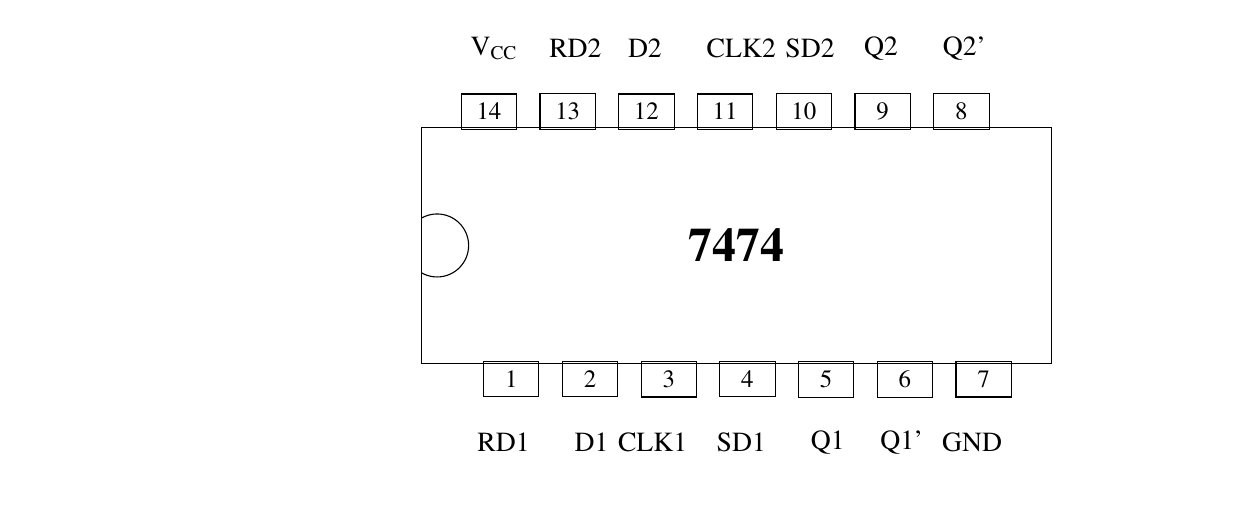
\begin{tikzpicture}[scale=1,
     pin/.style={draw,rectangle,minimum width=2em,font=\small}
     ]
   % Main trick: loop over the label numbers and then adjust their position
   % in the tikzpicture using evaluate to calculate \y=y-coordinate of pin

   \foreach \i/\desc [evaluate=\i  as \x using (\i+5 )]
      in {1/{RD1},
          2/{D1},
          3/{CLK1},
          4/{SD1},
          5/{Q1},
          6/{Q1'},
          7/{GND}}
   {
     \draw node[pin,anchor=east,rotate=360] at (\x+.5,-.2){\small$\i$};
     \node[align=right,anchor=east,rotate=360] at (\x+.5,-1){\desc};
   }
  
   \foreach \i/\desc [evaluate=\i as \x using (20-\i)]
      in {8/{Q2'},
          9/{Q2},
          10/{SD2},
          11/{CLK2},
          12/{D2},
          13/{RD2},
          14/{V$_{\text{CC}}$}}
   {
     \draw node[pin,anchor=west,rotate=360] at (\x-.5,3.2){\small$\i$};
     \node[align=right,anchor=west,rotate=360] at (\x-.5,4){\desc};
   }
   \draw
      (5,0.8)--(5,3)--(5,3)--(13,3)--(13,3)
             --(13,0.8)--(13,0)--(5,0)--cycle;
    \begin{scope}         
    \clip (15,.5) rectangle (5,2);         
   \draw(5.2,1.5)circle[radius=0.4];
   \end{scope}
   \begin{scope}
   \clip (0,-1.5) rectangle (1.5,1.5);
    \draw (2,) circle(6.5);
\end{scope}

   \node at (9,1.5){\textbf{\LARGE{7474}}};
 \end{tikzpicture}
\end{document}




}
\end{center}
\caption{}
\label{fig:7474}
\end{figure}

%
\begin{problem}
Intelligently use the codes in 
\begin{lstlisting}
wget https://raw.githubusercontent.com/gadepall/arduino/master/7447/codes/inc_dec/inc_dec.ino
\end{lstlisting}
and
\begin{lstlisting}
wget https://raw.githubusercontent.com/gadepall/arduino/master/7447/codes/ip_inc_dec/ip_inc_dec.ino
\end{lstlisting}
to realize the decade counter in Fig. \ref{fig:decade_counter}.
 \end{problem}
 
 \begin{figure}[!h]
\begin{center}
\resizebox {\columnwidth} {!} {
%\documentclass{article}

%\usepackage[latin1]{inputenc}
%\usepackage{tikz}
%\usetikzlibrary{shapes,arrows}

%%%%<
%\usepackage{verbatim}
%\usepackage[active,tightpage]{preview}
%\PreviewEnvironment{tikzpicture}
%\setlength\PreviewBorder{5pt}%
%%%%>

%\begin{comment}
%:Title: Simple flow chart
%:Tags: Diagrams

%With PGF/TikZ you can draw flow charts with relative ease. This flow chart from [1]_
%outlines an algorithm for identifying the parameters of an autonomous underwater vehicle model. 

%Note that relative node
%placement has been used to avoid placing nodes explicitly. This feature was
%introduced in PGF/TikZ >= 1.09.

%.. [1] Bossley, K.; Brown, M. & Harris, C. Neurofuzzy identification of an autonomous underwater vehicle `International Journal of Systems Science`, 1999, 30, 901-913 


%\end{comment}


%\begin{document}
%\pagestyle{empty}


% Define block styles
\tikzstyle{decision} = [diamond, draw, fill=blue!20, 
    text width=4.5em, text badly centered, node distance=3cm, inner sep=0pt]
%\tikzstyle{block} = [rectangle, draw, fill=blue!20, 
%    text width=5em, text centered, rounded corners, minimum height=4em]
\tikzstyle{block} = [rectangle, draw, 
    text width=5em, text centered, rounded corners, minimum height=4em]

\tikzstyle{line} = [draw, -latex']
\tikzstyle{cloud} = [draw, ellipse,fill=red!20, node distance=3cm,
    minimum height=2em]
    
\begin{tikzpicture}[node distance = 3cm, auto]
    % Place nodes
    \node [block] (init) {Incrementing Decoder};
%    \node [cloud, left of=init] (expert) {expert};
%    \node [cloud, right of=init] (system) {system};
    \node [block, below of=init, node distance = 4cm] (identify) {Display Decoder};
    \node [block, below of=identify ] (evaluate) {Seven-Segment Display};
%    \node [block, right of=identify, node distance = 4cm] (delay) {Delay};
     %\node [block, (4,-3)] (q1) {Delay};
	\node at (4,-2)[block] (delay) {Delay};
\begin{scope}[->,>=latex]
    \foreach \i in {-3,-1,1,3}
    { 
%      \draw[->] ([yshift=\i * 0.2 cm]identify.east) -- ([yshift=\i * 0.2 cm]delay.west) ;
      \draw[->] ([xshift=\i * 0.2 cm]delay.north) |- ([yshift=\i * 0.2 cm]init.east) ;
      \draw[->] ([xshift=\i * 0.2 cm]init.south) -- ([xshift=\i * 0.2 cm]identify.north) ;
       \draw node at (\i * 0.2,-2+\i * 0.2) { \textbullet} ;
       \draw[->] (\i * 0.2,-2+\i * 0.2) -- ([yshift=\i * 0.2 cm]delay.west) ;
      
    }
\foreach \i in {-3,...,3}
    { 
      \draw[->] ([xshift=\i * 0.35 cm]identify.south) -- ([xshift=\i * 0.35 cm]evaluate.north) ;
    }
\foreach [count=\i] \j in {a,b,...,g}{
            \node (\i) at ( 1.6-\i * 0.35, -5.5) {\j} ;
            }
\foreach [count=\i] \j in {A,B,C,D}{
            \node (\i) at ( 0.8-\i * 0.4, -1.0-\i*0.4) {\j} ;
            }

\foreach [count=\i] \j in {W,X,Y,Z}{
            \node (\i) at ( 1.6, 1.2-\i*0.4) {\j} ;
            }
    
\end{scope}

 %   \node [block, left of=evaluate, node distance=3cm] (update) {update model};
  %  \node [decision, below of=evaluate] (decide) {is best candidate better?};
%    \node [block, below of=decide, node distance=3cm] (stop) {stop};
    % Draw edges
%    \path [line] (init) -- (identify);
    \path [line] (identify) -- (evaluate);
%    \path [line] (evaluate) -- (decide);
  %  \path [line] (decide) -| node [near start] {yes} (update);
   % \path [line] (update) |- (identify);
 %   \path [line] (decide) -- node {no}(stop);
%    \path [line,dashed] (expert) -- (init);
%    \path [line,dashed] (system) -- (init);
%    \path [line,dashed] (system) |- (evaluate);
\end{tikzpicture}
%}

%\end{document}

}
\end{center}
\caption{}
\label{fig:decade_counter}
\end{figure}
%

\end{document}


